
\documentclass[11pt]{article}
\usepackage[a4paper, tmargin=0.75in, lmargin=0.80in, rmargin=0.80in, bmargin=1in]{geometry}

\usepackage{hyperref}
\usepackage{multicol}
\hypersetup{
    colorlinks=true,
    linkcolor=black,
    filecolor=magenta,      
    urlcolor=blue,
    citecolor=black,
}
%\usepackage[numbers,sort&compress]{natbib} % for a numerical citation list
\usepackage{natbib} % to cite references by surname and year
\usepackage{graphicx}
\usepackage{float}
\pagestyle{empty}


\usepackage{listings}
\usepackage{xcolor}
\usepackage{framed}

\usepackage[italian]{babel}

\lstset{
	basicstyle=\ttfamily\small,
	keywordstyle=\color{blue},
	commentstyle=\color{gray},
	stringstyle=\color{red},
	backgroundcolor=\color{gray!10},
	frame=single,
	breaklines=true,
	showstringspaces=false
}

\newcommand{\studentname}{Alessio Russo}
\newcommand{\studentnumber}{376856}
\newcommand{\course}{Scienze Informatiche}
\newcommand{\exam}{Modellazione e Simulazioni Numeriche}
%%%%%%%%%%%%%%%%%%%%%%%%%%%%%%%%%%%%%%%%%%%%%%%%%%
%%%%%%%%%%%%%%%%%%%%%%%%%%%%%%%%%%%%%%%%%%%%%%%%%%
%%%%%%%%%%%%%%%%%%%%%%%%%%%%%%%%%%%%%%%%%%%%%%%%%%
%%%%%%%%%%%%%%%%%%%%%%%%%%%%%%%%%%%%%%%%%%%%%%%%%%
%%%%%%%%%%%%%%%%%%%%%%%%%%%%%%%%%%%%%%%%%%%%%%%%%%
%%%%%%%%%%%%%%%%%%%%%%%%%%%%%%%%%%%%%%%%%%%%%%%%%%

\begin{document}


\begin{center}
{\Huge{Percolazione nei reticoli quadrati}} \\
%\vspace{2mm}
%{\Large{Relazione sul tema percolazione}} \\
%\vspace{2mm}
%{\Large{Alessio Russo}} \\
%\vspace{1mm}
%{\Large{Università degli studi di Parma}}
\end{center}

\vspace{5mm}
\hrule
\vspace{1mm}
\hrule
\vspace{3mm}
\begin{center}
	\begin{tabular}{llll}
		\textbf{Studente: } & {\studentname}  & \textbf{Matricola:}  & {\studentnumber}  \\ 
		\textbf{Corso di studio: } & {\course}& \textbf{Esame:} & {\exam}\\ 
	\end{tabular}
\end{center}
\vspace{3mm}
\hrule
\vspace{1mm}
\hrule

\section{Algoritmo di Hoshen-Kopelman}
L’algoritmo di Hoshen-Kopelman (HK76) è una tecnica di etichettatura multipla dei cluster. Il reticolo viene visitato sito per sito per colonne, partendo dallo spigolo in alto a sinistra per arrivare a quello in basso a destra. Si prenda, ad esempio, il reticolo
in figura
\begin{figure}[H]
	\centering
	\scriptsize % Riduce la dimensione del testo
	\setlength{\tabcolsep}{5.4pt} % Riduce lo spazio tra le colonne
	\renewcommand{\arraystretch}{1.3} % Riduce lo spazio verticale tra le righe
	\begin{minipage}{0.45\textwidth}
		\centering
		\begin{tabular}{|*{15}{c|}}
			\hline
			0 & 1 & 0 & 0 & 1 & 1 & 0 & 0 & 0 & 1 & 0 & 1 & 0 & 1 & 0 \\
			\hline
			0 & 1 & 1 & 0 & 0 & 0 & 1 & 0 & 0 & 1 & 1 & 1 & 1 & 1 & 1 \\
			\hline
			0 & 1 & 0 & 0 & 0 & 1 & 1 & 1 & 1 & 0 & 0 & 1 & 0 & 0 & 0 \\
			\hline
			1 & 0 & 1 & 0 & 1 & 0 & 1 & 0 & 0 & 0 & 1 & 1 & 0 & 0 & 0 \\
			\hline
			0 & 1 & 0 & 1 & 1 & 0 & 1 & 0 & 0 & 0 & 1 & 0 & 0 & 1 & 0 \\
			\hline
			0 & 0 & 1 & 1 & 1 & 1 & 1 & 0 & 1 & 1 & 1 & 1 & 1 & 0 & 1 \\
			\hline
			0 & 0 & 1 & 1 & 1 & 0 & 0 & 0 & 0 & 1 & 1 & 1 & 1 & 0 & 1 \\
			\hline
			0 & 1 & 0 & 1 & 1 & 1 & 1 & 0 & 1 & 1 & 1 & 1 & 0 & 1 & 0 \\
			\hline
			0 & 1 & 0 & 0 & 1 & 1 & 0 & 0 & 1 & 1 & 1 & 1 & 0 & 0 & 1 \\
			\hline
			1 & 0 & 0 & 0 & 0 & 0 & 0 & 0 & 1 & 0 & 0 & 0 & 0 & 1 & 0 \\
			\hline
			0 & 0 & 0 & 0 & 1 & 0 & 1 & 0 & 1 & 1 & 0 & 1 & 1 & 1 & 1 \\
			\hline
			1 & 1 & 0 & 0 & 0 & 1 & 0 & 1 & 0 & 1 & 1 & 1 & 1 & 1 & 1 \\
			\hline
			1 & 1 & 1 & 0 & 0 & 1 & 1 & 0 & 1 & 0 & 0 & 1 & 0 & 0 & 0 \\
			\hline
			0 & 1 & 0 & 1 & 1 & 1 & 1 & 1 & 0 & 1 & 1 & 1 & 0 & 1 & 1 \\
			\hline
			1 & 1 & 1 & 1 & 0 & 0 & 0 & 0 & 1 & 1 & 1 & 1 & 1 & 1 & 0 \\
			\hline
		\end{tabular}
	\end{minipage}
	\hfill
	\begin{minipage}{0.45\textwidth}
		\centering
		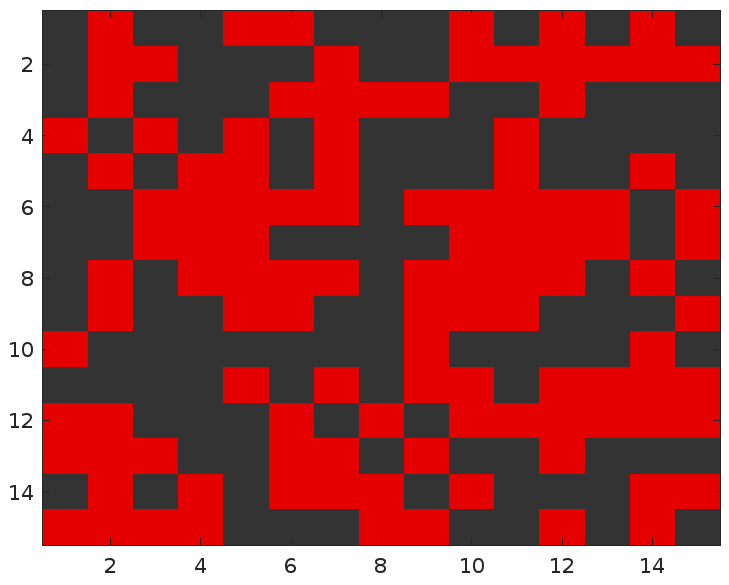
\includegraphics[width=\linewidth]{images/basegrid}
		\label{fig:basegrid}
	\end{minipage}
\end{figure}
\noindent
Durante la visita del reticolo, quando si incontra un sito colorato, allora: \textbf{(1)} Se il sito non è connesso ad altri siti colorato sopra o a sinistra, si inizia un nuovo cluster, a cui viene assegnata una \texttt{label} \textbf{(2)} Se c’è un primo vicino sopra o a sinistra colorato (uno solo dei due), il sito viene aggiunto al cluster del primo vicino colorato \textbf{(3)}Se i suoi primi vicini sono entrambi colorati, ma appartengono allo stesso cluster, il sito viene aggiunto al cluster dei primi vicini \textbf{(4)} Se i suoi primi vicini sono entrambi colorati, e non appartengono allo stesso cluster, il sito viene aggiunto al cluster con la \texttt{label} minore. Ad esempio, il cluster associati al reticolo precedente sono
mostrati in figura
\begin{figure}[H]
	\centering
	\scriptsize % Riduce la dimensione del testo
	\setlength{\tabcolsep}{3.5pt} % Riduce lo spazio tra le colonne
	\renewcommand{\arraystretch}{1.3} % Riduce lo spazio verticale tra le righe
	\begin{minipage}{0.4\textwidth}
		\centering
		\begin{center}
			\begin{tabular}{|*{15}{c|}}
				\hline
				0 & 1 & 0 & 0 & 2 & 2 & 0 & 0 & 0 & 3 & 0 & 4 & 0 & 5 & 0 \\
				\hline
				0 & 1 & 1 & 0 & 0 & 0 & 6 & 0 & 0 & 3 & 3 & 3 & 3 & 3 & 3 \\
				\hline
				0 & 1 & 0 & 0 & 0 & 7 & 6 & 6 & 6 & 0 & 0 & 3 & 0 & 0 & 0 \\
				\hline
				8 & 0 & 9 & 0 & 10 & 0 & 6 & 0 & 0 & 0 & 11 & 3 & 0 & 0 & 0 \\
				\hline
				0 & 12 & 0 & 13 & 10 & 0 & 6 & 0 & 0 & 0 & 11 & 0 & 0 & 14 & 0 \\
				\hline
				0 & 0 & 15 & 13 & 10 & 10 & 6 & 0 & 16 & 16 & 11 & 11 & 11 & 0 & 17 \\
				\hline
				0 & 0 & 15 & 13 & 10 & 0 & 0 & 0 & 0 & 16 & 11 & 11 & 11 & 0 & 17 \\
				\hline
				0 & 18 & 0 & 13 & 10 & 10 & 10 & 0 & 19 & 16 & 11 & 11 & 0 & 20 & 0 \\
				\hline
				0 & 18 & 0 & 0 & 10 & 10 & 0 & 0 & 19 & 16 & 11 & 11 & 0 & 0 & 21 \\
				\hline
				22 & 0 & 0 & 0 & 0 & 0 & 0 & 0 & 19 & 0 & 0 & 0 & 0 & 23 & 0 \\
				\hline
				0 & 0 & 0 & 0 & 24 & 0 & 25 & 0 & 19 & 19 & 0 & 26 & 26 & 23 & 23 \\
				\hline
				27 & 27 & 0 & 0 & 0 & 28 & 0 & 29 & 0 & 19 & 19 & 19 & 19 & 19 & 19 \\
				\hline
				27 & 27 & 27 & 0 & 0 & 28 & 28 & 0 & 30 & 0 & 0 & 19 & 0 & 0 & 0 \\
				\hline
				0 & 27 & 0 & 31 & 31 & 28 & 28 & 28 & 0 & 32 & 32 & 19 & 0 & 33 & 33 \\
				\hline
				34 & 27 & 27 & 27 & 0 & 0 & 0 & 0 & 35 & 32 & 32 & 19 & 19 & 19 & 0 \\
				\hline
			\end{tabular}
		\end{center}
	\end{minipage}
	\hfill
	\begin{minipage}{0.45\textwidth}
		\centering
		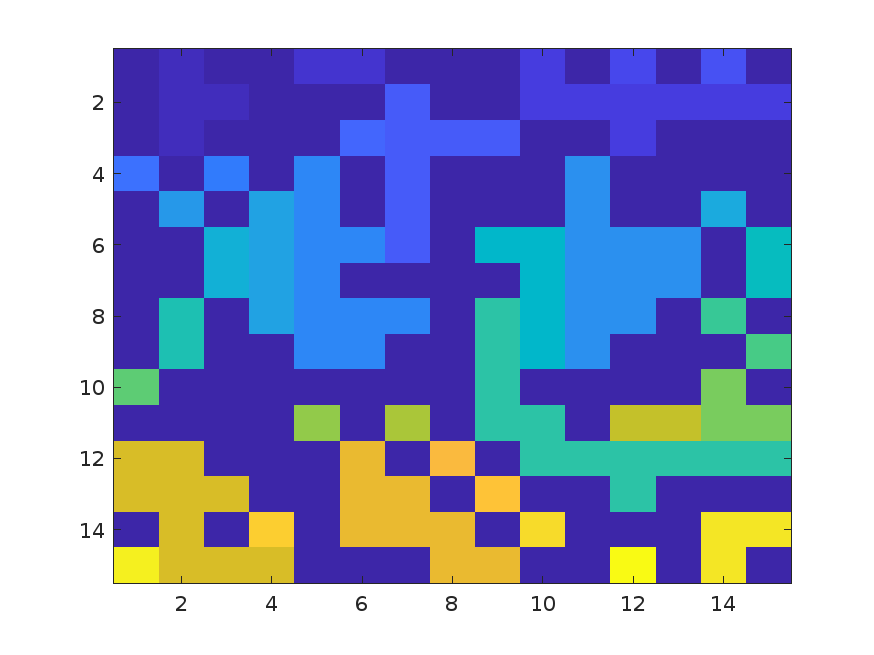
\includegraphics[width=\linewidth]{images/labels}
		\label{fig:basegrid}
	\end{minipage}
\end{figure}
\noindent
Tuttavia, quando si incontra un caso come quello descritto nel punto \textbf{(4)}, occorre  memorizzare che i due cluster sono in realtà lo stesso cluster. Questo viene fatto usando un vettore chiamato \textbf{Label of Label} (\texttt{LofL}), che contiene tutta l’informazione necessaria sui label dei cluster. In particolare, il modulo \texttt{HKclass}: 
per un \textit{good label}, memorizza la taglia del cluster; 
per \textit{bad label}, memorizza qual è il vero cluster label a cui questo label appartiene.  Questa distinzione viene fatta attraverso i segni dei numeri interi contenuti in LofL. Di seguito è riportato il LofL corrispondete al reticolo preso in esame

\vspace{15px}
\noindent
\begin{tabular}{|c|*{12}{c|}}
	\hline
	\textbf{ID}   & 1 & 2 & 3 & 4 & 5 & 6 & 7 & 8 & 9 & 10 & 11 & 12 \\
	\hline
	\textbf{Val}  & 4 & 2 & 56 & -3 & -3 & 24 & -6 & 1 & 1 & -6 & -3 & 1 \\
	\hline
\end{tabular}

\vspace{10px}
\noindent
\begin{tabular}{|c|*{12}{c|}}
	\hline
	\textbf{ID}   & 13 & 14 & 15 & 16 & 17 & 18 & 19 & 20 & 21 & 22 & 23 & 24 \\
	\hline
	\textbf{Val}  & -10 & 1 & -10 & -3 & 2 & 2 & -3 & 1 & 1 & 1 & -3 & 1 \\
	\hline
\end{tabular}

\vspace{10px}
\noindent
\begin{tabular}{|c|*{11}{c|}}
	\hline
	\textbf{ID}   & 25 & 26 & 27 & 28 & 29 & 30 & 31 & 32 & 33 & 34 & 35 \\
	\hline
	\textbf{Val}  & 1 & -3 & 18 & -27 & 1 & 1 & -27 & -3 & -3 & -27 & -3 \\
	\hline
\end{tabular}

\vspace{15px}
\noindent
Tuttavia, l’algoritmo HK restituisce in modo corretto le taglie dei cluster, ma non garantisce che tutti i siti di un fissato cluster abbiano lo stesso valore. Per questo motivo, al fine di identificare la presenza di cluster percolanti, effettuiamo una rilabelizzazione successiva. Di seguito ne è mostrato un esempio.

\begin{figure}[H]
	\centering
	\scriptsize % Riduce la dimensione del testo
	\setlength{\tabcolsep}{3.5pt} % Riduce lo spazio tra le colonne
	\renewcommand{\arraystretch}{1.3} % Riduce lo spazio verticale tra le righe
	\begin{minipage}{0.4\textwidth}
		\centering
		\begin{center}
			\begin{tabular}{|*{15}{c|}}
				\hline
				0 & 1 & 0 & 0 & 2 & 2 & 0 & 0 & 0 & 3 & 0 & 3 & 0 & 3 & 0 \\
				\hline
				0 & 1 & 1 & 0 & 0 & 0 & 6 & 0 & 0 & 3 & 3 & 3 & 3 & 3 & 3 \\
				\hline
				0 & 1 & 0 & 0 & 0 & 6 & 6 & 6 & 6 & 0 & 0 & 3 & 0 & 0 & 0 \\
				\hline
				8 & 0 & 9 & 0 & 6 & 0 & 6 & 0 & 0 & 0 & 3 & 3 & 0 & 0 & 0 \\
				\hline
				0 & 12 & 0 & 6 & 6 & 0 & 6 & 0 & 0 & 0 & 3 & 0 & 0 & 14 & 0 \\
				\hline
				0 & 0 & 6 & 6 & 6 & 6 & 6 & 0 & 3 & 3 & 3 & 3 & 3 & 0 & 17 \\
				\hline
				0 & 0 & 6 & 6 & 6 & 0 & 0 & 0 & 0 & 3 & 3 & 3 & 3 & 0 & 17 \\
				\hline
				0 & 18 & 0 & 6 & 6 & 6 & 6 & 0 & 3 & 3 & 3 & 3 & 0 & 20 & 0 \\
				\hline
				0 & 18 & 0 & 0 & 6 & 6 & 0 & 0 & 3 & 3 & 3 & 3 & 0 & 0 & 21 \\
				\hline
				22 & 0 & 0 & 0 & 0 & 0 & 0 & 0 & 3 & 0 & 0 & 0 & 0 & 3 & 0 \\
				\hline
				0 & 0 & 0 & 0 & 24 & 0 & 25 & 0 & 3 & 3 & 0 & 3 & 3 & 3 & 3 \\
				\hline
				27 & 27 & 0 & 0 & 0 & 27 & 0 & 29 & 0 & 3 & 3 & 3 & 3 & 3 & 3 \\
				\hline
				27 & 27 & 27 & 0 & 0 & 27 & 27 & 0 & 30 & 0 & 0 & 3 & 0 & 0 & 0 \\
				\hline
				0 & 27 & 0 & 27 & 27 & 27 & 27 & 27 & 0 & 3 & 3 & 3 & 0 & 3 & 3 \\
				\hline
				27 & 27 & 27 & 27 & 0 & 0 & 0 & 0 & 3 & 3 & 3 & 3 & 3 & 3 & 0 \\
				\hline
			\end{tabular}
		\end{center}
	\end{minipage}
	\hfill
	\begin{minipage}{0.45\textwidth}
		\centering
		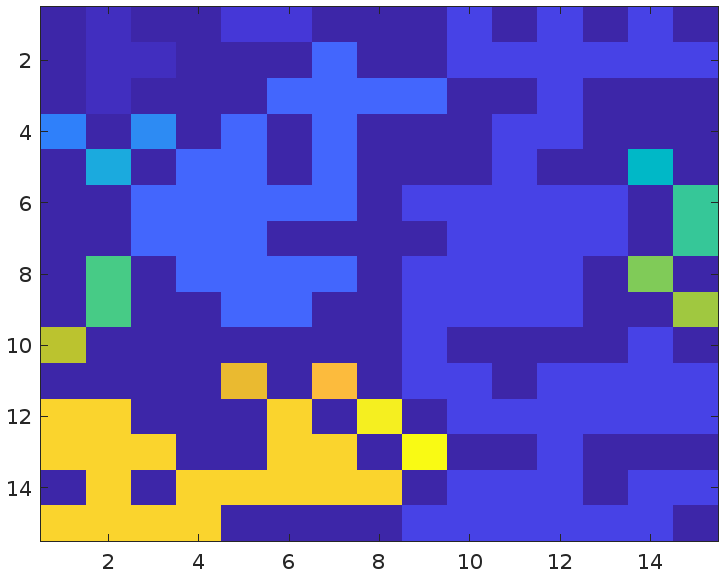
\includegraphics[width=\linewidth]{images/re-labelled}
		\label{fig:basegrid}
	\end{minipage}
\end{figure}
\noindent
A questo punto, l'obiettivo è determinare se esistono cluster percolanti all'interno del reticolo, ossia se esiste almeno un'etichetta condivisa tra la prima e l'ultima riga (percolazione verticale) e tra la prima e l'ultima colonna (percolazione orizzontale). Per fare ciò, possiamo sviluppare un algoritmo che, basandosi sull'estrazione delle etichette \textbf{uniche} presenti lungo i bordi della matrice, e mediante l'utilizzo dell'operazione \texttt{intersect},  verifica l'esistenza di almeno una etichetta comune tra i bordi opposti. Se tale etichetta è presente, viene restituito \texttt{true} per il tipo di percolazione considerato, altrimenti \texttt{false}.
\\\\
\noindent
Tuttavia, poiché ci interessa esclusivamente determinare il cluster di appartenenza della prima e dell’ultima riga e colonna per valutare la percolazione, è sufficiente rilabelare solo questi elementi, ignorando il centro del reticolo e risparmiando così tempo di calcolo. La Figura \ref{fig:relabelled-edge} ne mostra un esempio.
\begin{figure}
	\centering
	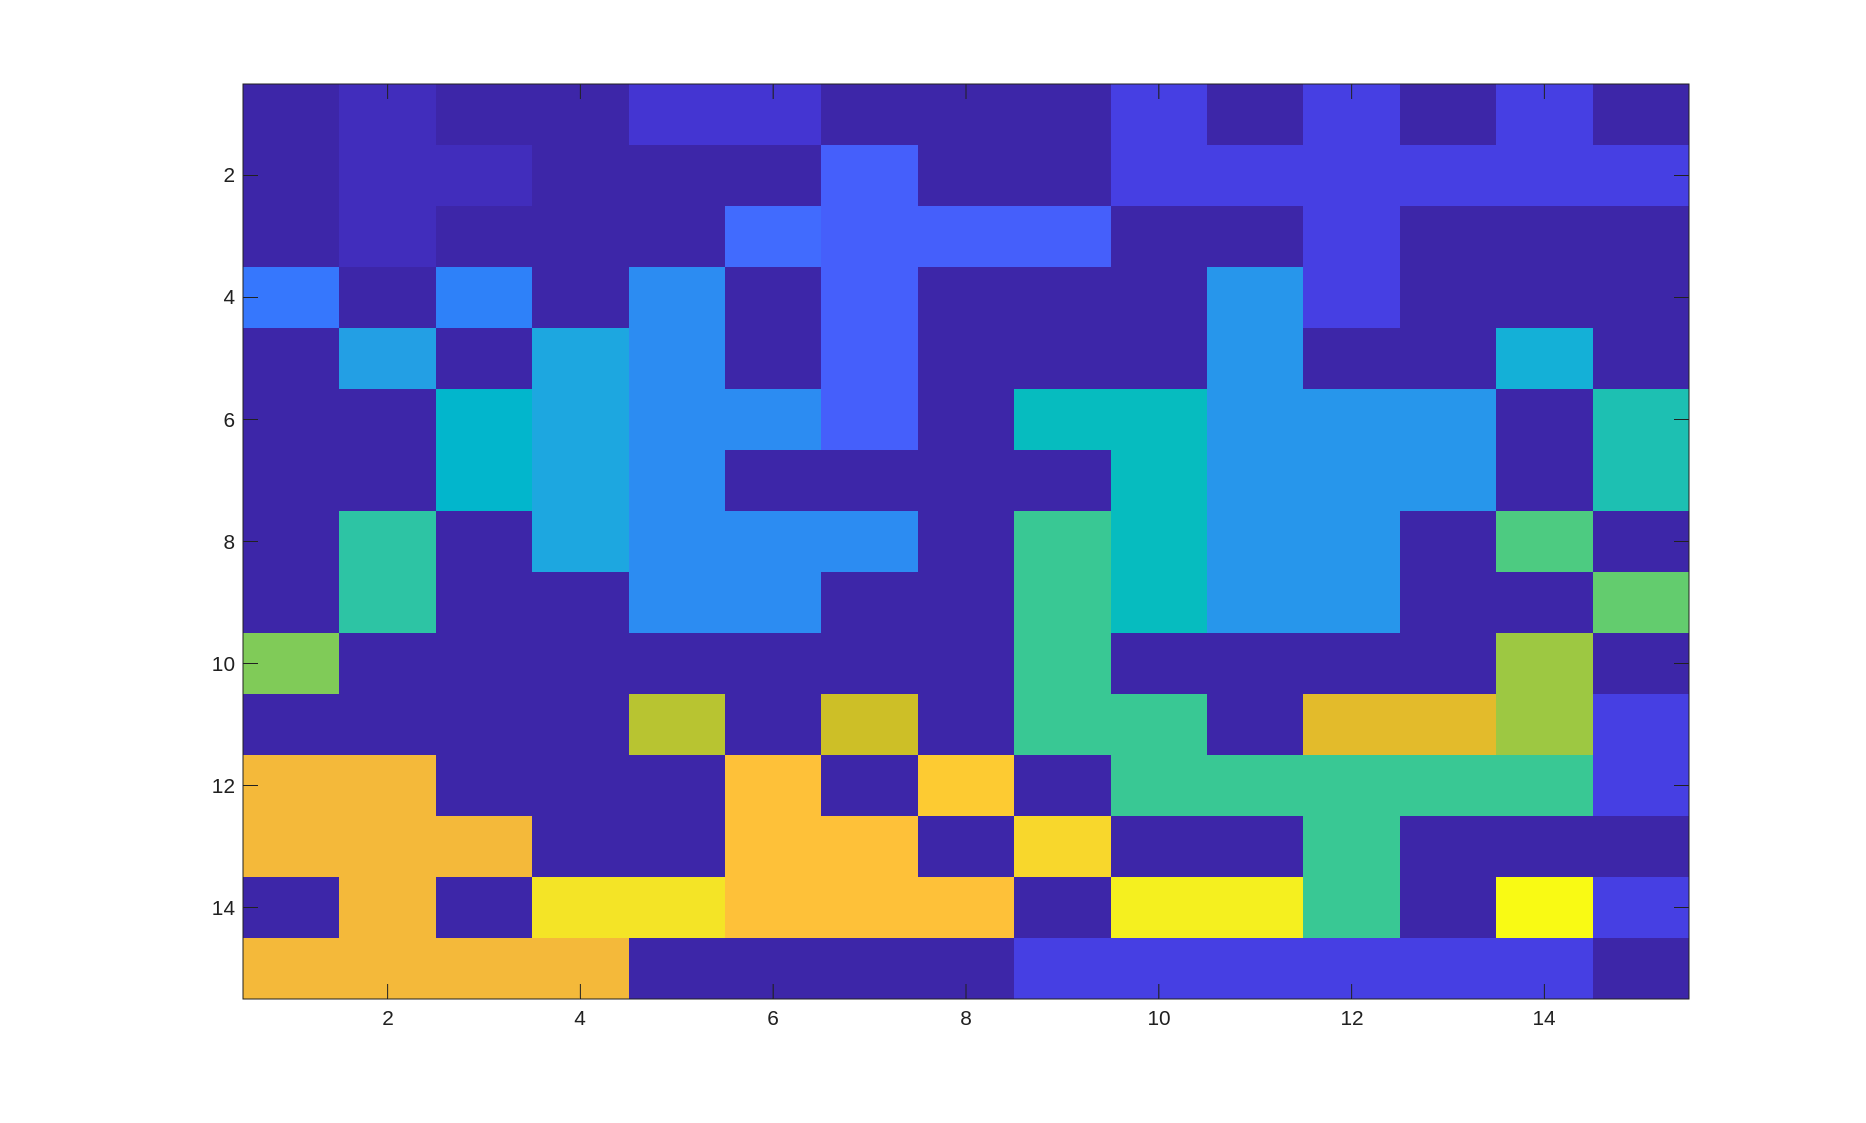
\includegraphics[width=0.7\linewidth]{images/re-labelled-edge}
	\caption{Esempio di ri-labeling limitato ai bordi del reticolo}
	\label{fig:relabelled-edge}
\end{figure}
\\\\
\noindent
Concludiamo dicendo che l'analisi della correttezza dell'implementazione proposta è stata effettuata non soltanto tramite test individuali sul singolo algoritmo, ma anche attraverso un confronto diretto con l'algoritmo naive presentato a lezione. Nello specifico, è stato generato un reticolo bidimensionale di dimensioni $100 \times 100$, con una probabilità di colorazione dei siti pari al 50\%. Tale reticolo è stato analizzato prima con l'algoritmo naive e successivamente con l'algoritmo HK76, confrontando i risultati ottenuti per la percolazione verticale (top-bottom) e orizzontale (left-right). Questo confronto è stato ripetuto $10.000$ volte, e in tutti i casi i risultati forniti dai due algoritmi sono stati coincidenti. 
\section{Confronto tra algoritmi naive e HK76}

L'algoritmo di Hoshen-Kopelman (HK76, indicato in \textit{blu}) ha mostrato una significativa efficienza computazionale superiore rispetto all'algoritmo di etichettatura naive (indicato in \textit{arancione}), precedentemente implementato. Questa valutazione è stata condotta attraverso due diverse analisi: la prima ha considerato il tempo di calcolo mantenendo costante la probabilità di colorazione dei siti e variando la dimensione del reticolo, mentre la seconda ha studiato il comportamento opposto, ovvero il tempo di calcolo mantenendo costante la dimensione del reticolo e variando la probabilità di colorazione dei siti.
\begin{figure}[H]
	\centering
	\includegraphics[width=0.7\linewidth]{images/compare\_t}
	\caption{Tempo di esecuzione in funzione della dimensione del reticolo per gli algoritmi HK76 e naive.}
	\label{fig:comparet}
\end{figure}
\subsection{Confronto con probabilità costante e taglia variabile}
Nel primo caso, è stata fissata una probabilità di colorazione dei siti pari al $60\%$, variando la dimensione del reticolo quadrato nell'intervallo compreso tra $100$ e $1000$, con incrementi di $100$, per un totale di $10$ configurazioni. La Figura \ref{fig:comparet} mostra i tempi medi di esecuzione dell'algoritmo, calcolati eseguendo ciascuna configurazione 50 volte. Si noti come, all’aumentare della dimensione del reticolo, l’algoritmo HK76 offra prestazioni migliori rispetto all’algoritmo naive in termini di tempo di esecuzione. Di seguito sono riportati i tempi medi di esecuzione:

\vspace{15px}
\noindent
\begin{tabular}{|c|*{10}{c|}}
	\hline
	\textbf{hk76} &0.0005 &	0.0018 &	0.0037 &	0.0065 &	0.0099 &	0.0140 &	0.0192 &	0.0255 &	0.0313 &	0.0385 \\
	\hline
	\textbf{naive} & 0.0023  &  0.0090  &  0.0199 &   0.0354 &   0.0552  &  0.0806 &   0.1097  &  0.1482 &   0.1877  &  0.2383\\
	\hline
\end{tabular}

\vspace{15px}
\noindent
e i relativi errori (da moltiplicare per $10^{-3}$):

\vspace{15px}
\noindent
\begin{tabular}{|c|*{10}{c|}}
	\hline
	\textbf{hk76}  & 0.0107  &  0.0511    &0.0261 &   0.0830   & 0.1095   & 0.1083  &  0.1271  &  0.1536  &  0.1598  &  0.1649\\
	\hline
	\textbf{naive}  &0.0108  &  0.0224  &  0.0177  &  0.1090  &  0.1216  &  0.2112   & 0.2641  &  0.2072&    0.3270  &  0.4488\\
	\hline
\end{tabular}

\subsection{Confronto con taglia costante e probabilità variabile}
Nel secondo caso, invece, la dimensione del reticolo è stata mantenuta fissa a $500$, mentre la probabilità di colorazione dei siti è stata variata da $0{,}1$ a $1$, con incrementi di $0{,}1$, per un totale di $10$ esperimenti. 
\begin{figure}[H]
	\centering
	\includegraphics[width=0.7\linewidth]{images/compare\_p}
	\caption{Tempo di esecuzione in funzione della probabilità di colorazione per gli algoritmi HK76 e naive.}
	\label{fig:comparep}
\end{figure}
\noindent
La Figura \ref{fig:comparep}, che mostra i tempi medi di esecuzione su $50$ iterazioni, evidenzia come l’algoritmo HK76 risulti nettamente migliore rispetto alla versione naive. Di seguito sono riportati i tempi medi di esecuzione:

\vspace{15px}
\noindent
\begin{tabular}{|c|*{10}{c|}}
	\hline
	\textbf{hk76} &0.0032 &   0.0047 &   0.0063  &  0.0076 &   0.0087   &  0.0110   & 0.0497  &  0.0327    &0.0086    & 0.0061 \\
	\hline
	\textbf{naive} &0.0120 &   0.0242 &   0.0377   & 0.0480  &  0.0544 &   0.0600  &  0.0643  &  0.0688 &   0.0762 &   0.0845
	\\
	\hline
\end{tabular}

\vspace{15px}
\noindent
e i relativi errori (da moltiplicare per $10^{-3}$):

\vspace{15px}
\noindent
\begin{tabular}{|c|*{10}{c|}}
	\hline
	\textbf{hk76}  & 0.0776  &  0.0643 &   0.0935 &   0.0997&    0.0864  &  0.1096   & 0.6884  &  0.4468&    0.0981  &  0.0650\\
	\hline
	\textbf{naive}  & 0.1488  &  0.2100 &   0.4623  &  0.4539 &   0.3350  &  0.4271 &   0.2585  &  0.2870 &   0.2396 &   0.3537\\
	\hline
\end{tabular}

\vspace{15px}
\noindent
\section{Ricerca della soglia di percolazione}
Per analizzare il comportamento della probabilità di percolazione $P_{perc}$ in funzione della probabilità di occupazione dei siti $p_{col}$, è stata condotta una serie di simulazioni su reticoli quadrati di diverse dimensioni ($L = 100$, $300$ e $1000$). L’intervallo di $p_{col}$ considerato va da $0.55$ a $0.65$, con incrementi di $0.01$, in modo da esplorare con buona risoluzione la zona critica.
\\\\
\noindent
Per ogni coppia di valori $(L, p_{col})$, l’esperimento è stato ripetuto $50$ volte, così da permettere una stima della probabilità di percolazione e del relativo errore. Ogni simulazione consiste nella generazione di un reticolo in cui ogni sito viene occupato con probabilità $p_{col}$. Una volta creato il reticolo, i cluster connessi di siti occupati sono stati individuati tramite l'algoritmo hk76. Successivamente, è stato verificato se esiste almeno un cluster che attraversa il reticolo da sinistra a destra (percolazione orizzontale) o dall’alto in basso (percolazione verticale).
\\\\
\noindent
Un confronto tra i risultati ottenuti nelle due direzioni ha permesso di confermare che, come previsto, tenendo conto dei relativi errori, la probabilità di percolazione orizzontale è la stessa di quella verticale.
\\\\
\textbf{Probabilità media di percolazione LR}
\\\\
\noindent
\begin{tabular}{|c|*{11}{c|}}
	\hline
	\textbf{}&\textbf{0.55} &	\textbf{0.56}& \textbf{0.57} &	\textbf{0.58}	& \textbf{0.59}& 	\textbf{0.60}&	\textbf{0.61}&\textbf{	0.62}&	\textbf{0.63}& \textbf{0.64} &\textbf{0.65}	\\
	\hline
	
	\textbf{100} &0.02 &	0.06& 0.06 &	0.18	& 0.38& 	0.60&	0.90&	0.94&	1.00 &	1.00 &	1.00\\
	\hline

	\textbf{300} & 0.00	& 0.00	& 0.00&	0.00&	0.30 & 0.82 &	0.98&	1.00&1.00&1.00&1.00\\
	\hline
	\textbf{1000}& 0.00&	0.00	&0.00	&0.00	&0.16&	0.98&	1.00&	1.00 & 1.00 & 1.00 & 1.00\\
	\hline
\end{tabular}
\vspace{15px}

\noindent
\textbf{Probabilità media di percolazione TB}

\vspace{15px}
\noindent
\begin{tabular}{|c|*{11}{c|}}
	\hline
	\textbf{}&\textbf{0.55} &	\textbf{0.56}& \textbf{0.57} &	\textbf{0.58}	& \textbf{0.59}& 	\textbf{0.60}&	\textbf{0.61}&\textbf{	0.62}&	\textbf{0.63}& \textbf{0.64} &\textbf{0.65}	\\
	\hline
	
	\textbf{100} &0.00 &	0.06 & 0.10	& 0.18	&0.48&	0.70&	0.82& 0.90&	1.00&	1.00&	1.00\\
	\hline
	\textbf{300}& 0.00	&0.00	&0.00	&0.02&	0.36&	0.86&	0.98&	1.00&	1.00	&1.00&	1.00 \\
	\hline
	\textbf{1000}&0.00	&0.00	&0.00	&0.00	&0.18&	1.00	&1.00	&1.00	&1.00&	1.00&	1.00\\
	\hline
\end{tabular}
\vspace{15px}

\noindent
\textbf{Errore nel calcolo di LR}

\vspace{15px}
\noindent
\begin{tabular}{|c|*{11}{c|}}
	\hline
	\textbf{} & \textbf{0.55} & \textbf{0.56} & \textbf{0.57} & \textbf{0.58} & \textbf{0.59} & \textbf{0.60} & \textbf{0.61} & \textbf{0.62} & \textbf{0.63} & \textbf{0.64} & \textbf{0.65} \\
	\hline
	\textbf{100}  & 0.02 & 0.03 & 0.03 & 0.05 & 0.07 & 0.07 & 0.04 & 0.03 & 0.00 & 0.00 & 0.00 \\
	\hline
	\textbf{300}  & 0.00 & 0.00 & 0.00 & 0.00 & 0.07 & 0.05 & 0.02 & 0.00 & 0.00 & 0.00 & 0.00 \\
	\hline
	\textbf{1000} & 0.00 & 0.00 & 0.00 & 0.00 & 0.05 & 0.02 & 0.00 & 0.00 & 0.00 & 0.00 & 0.00 \\
	\hline
\end{tabular}
\vspace{15px}

\noindent
\textbf{Errore nel calcolo di TB}

\vspace{15px}
\noindent
\begin{tabular}{|c|*{11}{c|}}
	\hline
	\textbf{} & \textbf{0.55} & \textbf{0.56} & \textbf{0.57} & \textbf{0.58} & \textbf{0.59} & \textbf{0.60} & \textbf{0.61} & \textbf{0.62} & \textbf{0.63} & \textbf{0.64} & \textbf{0.65} \\
	\hline
	\textbf{100}  & 0.00 & 0.03 & 0.04 & 0.05 & 0.07 & 0.07 & 0.05 & 0.04 & 0.00 & 0.00 & 0.00 \\
	\hline
	\textbf{300}  & 0.00 & 0.00 & 0.00 & 0.02 & 0.07 & 0.05 & 0.02 & 0.00 & 0.00 & 0.00 & 0.00 \\
	\hline
	\textbf{1000} & 0.00 & 0.00 & 0.00 & 0.00 & 0.05 & 0.00 & 0.00 & 0.00 & 0.00 & 0.00 & 0.00 \\
	\hline
\end{tabular}

\vspace{15px}
\noindent
Per ogni dimensione del reticolo $L$ è stata stimata la soglia di percolazione $p_c$ come il valore della probabilità di colorazione $p_{col}$ per cui la probabilità di percolazione $P_{perc}$ raggiunge il valore $0.5$.
\\\\
\noindent
Poiché i dati ottenuti tramite simulazione possono contenere duplicati (ad esempio valori estremi come $0.00$ e $1.00$), sono stati innanzitutto rimossi i punti ripetuti nei valori di $P_{perc}$.

\begin{figure}[H]
	\centering
	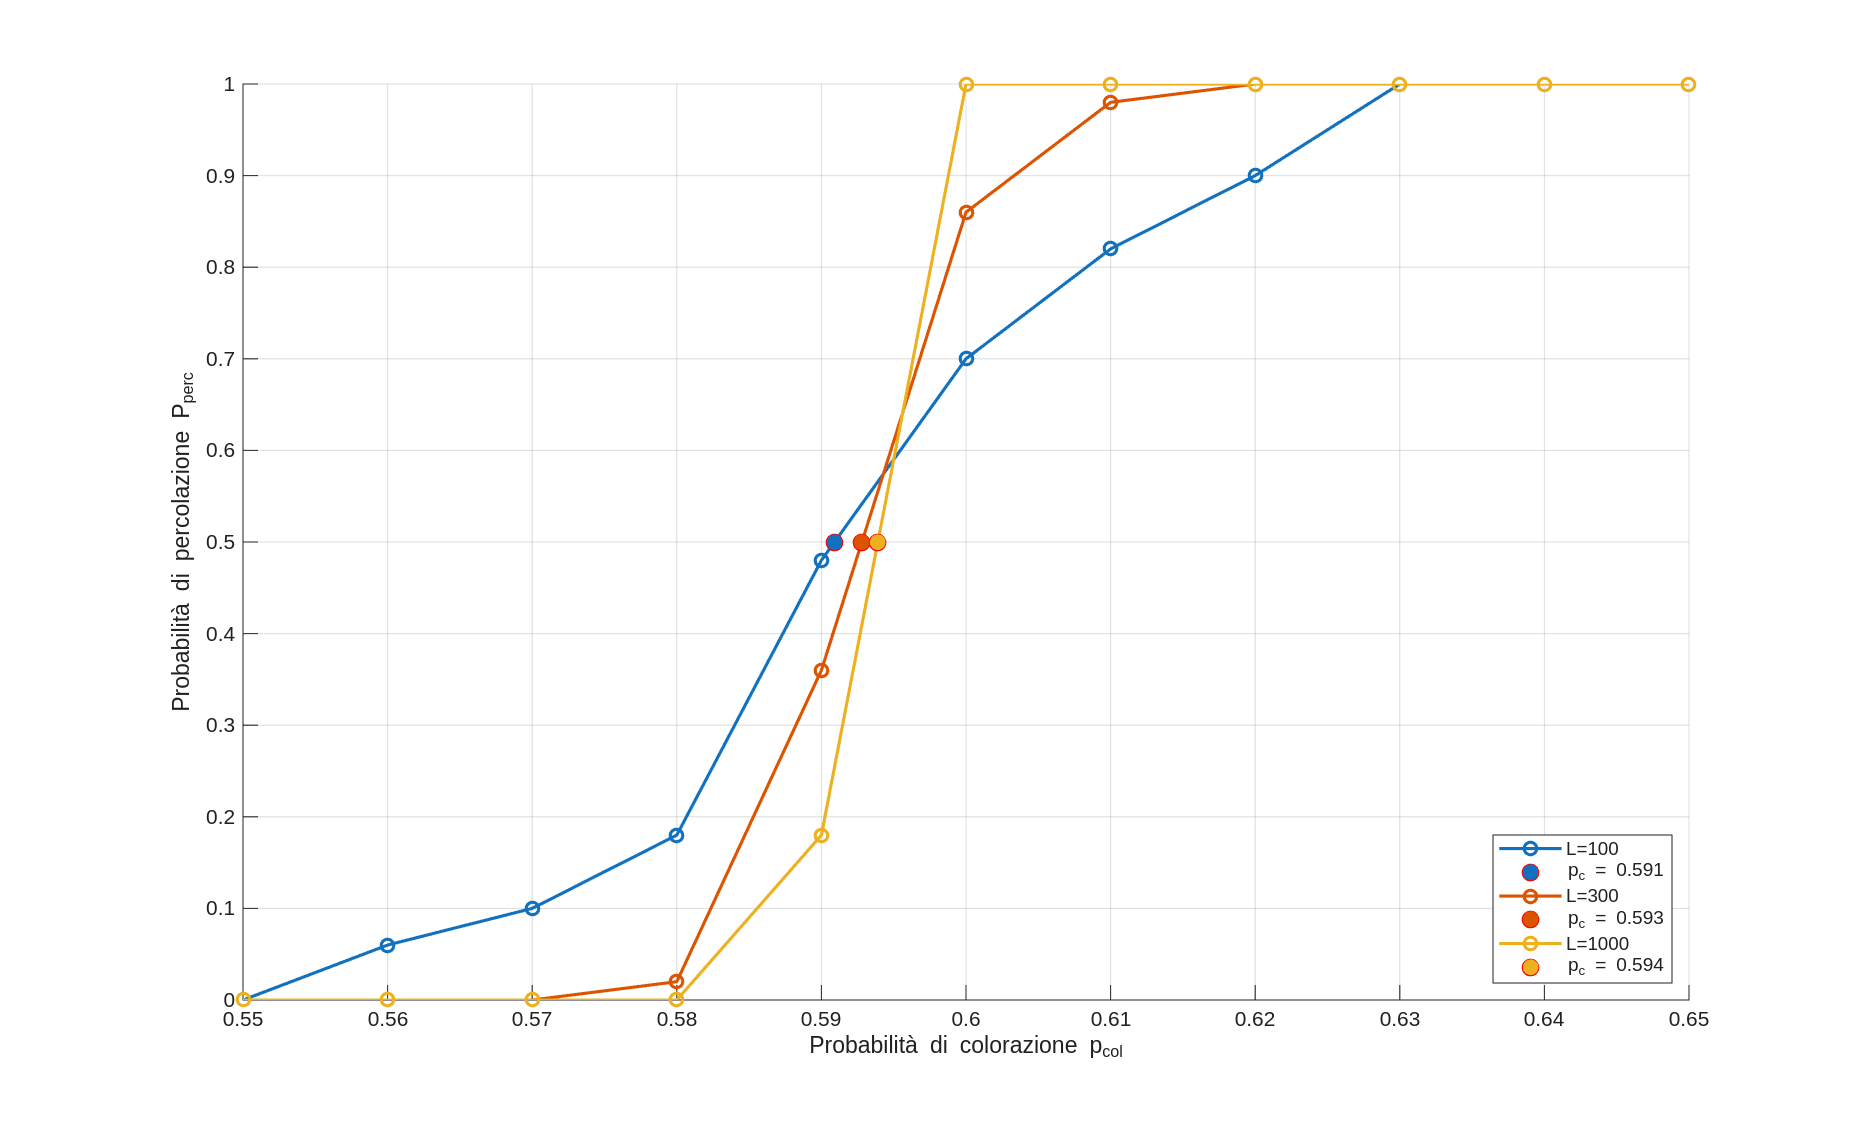
\includegraphics[width=\linewidth]{images/percolation_threshold.png}
	\caption{Andamento della probabilità di percolazione al variare di $p_{col}$.}
	\label{fig:perc_thr}
\end{figure}

\noindent
Successivamente, è stata utilizzata un’interpolazione lineare tra i punti ottenuti per stimare il valore di $p_{col}$ tale che $P_{perc} = 0.5$. Per ciascuna taglia del reticolo, il valore stimato di $p_c$ è stato evidenziato nel grafico in Figura~\ref{fig:perc_thr} come punto pieno sovrapposto alla curva $P_{perc}(p_{col})$. La procedura è stata ripetuta per tutte le dimensioni considerate, in modo da ottenere una stima della soglia di percolazione in funzione di $L$.
\\\\
\noindent
Questo approccio consente anche di osservare l’avvicinamento di $p_c(L)$ al valore critico nel limite termodinamico. In particolare, sulla base dei risultati ottenuti, questo valore asintotico è stimato attorno a $p_c \sim 0.59$.




\end{document}